\documentclass[11pt, a4paper]{article}
\usepackage[norsk]{babel}

%For fill text
\usepackage{blindtext}

%For linenumbers
\usepackage{lineno}

%For references
\usepackage{natbib}
\bibliographystyle{abbrvnat}
\usepackage[hidelinks,
            pdfauthor={
                          Skriv in forfatter her,~
                            Skriv in forfatter her,~
                            Skriv in forfatter her,~
                            Skriv in forfatter her,~
                          },
            pdftitle={Skriv in titell nivå 1 her},
            pdfsubject={Skriv in titell nivå 2 her},
            pdfkeywords={
                            geografisk område (land, fylke, kommune),~
                            art (fauna, flora, høyere taksonomisk enhet,~
                            konsekvensutredning,~
                            overvåkingsrapport,~
                            etterundersøkelse,~
                            vassdrag,~
                            økosystemtjenester,~
                            radioaktivitet,~
                          }]{hyperref}


%For getting total pagecount
\usepackage{lastpage}

%To get pdf production date in proper format
\usepackage[norsk]{datetime}
\newdateformat{ninadate}{%
\monthname[\THEMONTH]~ \THEYEAR}

%Set fonts
\usepackage{fontspec}
\setmainfont{Arial}
\newfontfamily{\narrow}{Arial Narrow}
\newfontfamily{\narrowbold}{Arial Narrow Bold}

%To insert manual hyphens
\usepackage{hyphenat}

%To refer to sections, figures and tables
\usepackage{nameref}
\newcommand*{\myref}[1]{\hyperref[{#1}]{\autoref*{#1} \nameref*{#1}}}

%Modify table of contents style
%\usepackage{titlesec}
\usepackage{titletoc}
\setcounter{tocdepth}{2}
\contentsmargin{0pt}
\dottedcontents{section}[2.3em]{\bfseries}{2.3em}{5pt}
\usepackage{setspace}

%To adjust margins and use left justification
\usepackage[a4paper, left=1.5cm,right=3.5cm,top=2cm,bottom=2cm,headheight=1cm]{geometry}
\usepackage[document]{ragged2e}

%To adjust heading spacings
\usepackage{titlesec}
\titlespacing\subsection{0pt}{12pt plus 4pt minus 2pt}{0pt plus 2pt minus 2pt}
\newcommand{\smallspace}{\vspace{3mm}}
\newcommand{\medspace}{\vspace{5mm}}

%Adjust paragraph indentations
\setlength{\parindent}{0pt}

%To adjust graphics
\usepackage{graphicx}
%\usepackage{epstopdf}


%Modify headers and footers
\usepackage{fancyhdr}
\pagestyle{fancy}
\addtolength{\headheight}{2pt}
\renewcommand{\headrulewidth}{0pt}
\renewcommand{\footrulewidth}{0pt}

%Defines the line in the pagefooter
\newcommand*\ruleline[1]{\par\noindent\raisebox{.4ex}{\makebox[\linewidth]{\hrulefill\hspace{1ex}\raisebox{-.4ex}{#1}\hspace{1ex}\hrulefill}}}

%Define titlepage footer
\usepackage{tikzpagenodes}
\fancypagestyle{titlefooter}{% Define title footer (change to svg logo)
  \fancyhf{}
  \lfoot{\vspace{1cm}\hspace{-1cm}
\includegraphics[height=2cm]{logo.eps}}
   \rfoot{\vspace{2.5cm}\hfill\Large\darkGrey{\narrow{Norsk institutt for naturforskning}}}
    \begin{tikzpicture}[remember picture,overlay]
  \fill[footgrey]
    (current page.south west)
    rectangle
  (current page.east|-current page footer area.south east);
  \end{tikzpicture}
}

%Define endpage footer
\fancypagestyle{endfooter}{% Define endpage footer (change to svg logo)
  \fancyhf{}
  \fancyfootoffset[R]{0cm}
  \begin{center}
  \vfill{}ISSN: 2464-2797 \\
ISBN: 978-82-426-1234-5
\end{center}
  \lfoot{\color{darkgrey}\vspace{1.5cm}\Large\narrow{\textbf{Norsk institutt for naturforskning}}\\
\begingroup
\narrow
\large NINA Hovedkontor\\
Postadresse: Postboks 5685 Sluppen, 7485 Trondheim\\
Besøks-/leveringsadresse: Høgskoleringen 9, 7034 Trondheim\\
Telefon: 73 80 14 00, Telefaks: 73 80 14 01\\
E-post: firmapost@nina.no\\
Organisasjonsnummer 9500 37 687\\
http://www.nina.no
\endgroup}
   \rfoot{\vspace{5cm}\hfill\Large\darkGrey{\narrow{Samarbeid og kunnskap for framtidas miljøløsninger}}}
    \begin{tikzpicture}[remember picture,overlay]
  \fill[footgrey]
    (current page.south west)
    rectangle
  (current page.east|-current page footer area.south east);
  \end{tikzpicture}
}

%Make sure it always produce even numbered document (adding empty page if necessary)
\usepackage{scrextend}
\newcommand{\OpenNewPageIfNeeded}{%
  \ifthispageodd{\fancyhf{}\newgeometry{a4paper, bottom=8cm, top=2cm, left=1.5cm, right=1.5cm}\null\clearpage~\pagestyle{endfooter}
  }{\fancyhf{}\newgeometry{a4paper, bottom=8cm, top=2cm, left=1.5cm, right=1.5cm}\null\pagestyle{endfooter}}
}
\AtEndDocument{\OpenNewPageIfNeeded}


\usepackage{color}
\usepackage{fancyvrb}
\newcommand{\VerbBar}{|}
\newcommand{\VERB}{\Verb[commandchars=\\\{\}]}
\DefineVerbatimEnvironment{Highlighting}{Verbatim}{commandchars=\\\{\}}
% Add ',fontsize=\small' for more characters per line
\usepackage{framed}
\definecolor{shadecolor}{RGB}{248,248,248}
\newenvironment{Shaded}{\begin{snugshade}}{\end{snugshade}}
\newcommand{\KeywordTok}[1]{\textcolor[rgb]{0.13,0.29,0.53}{\textbf{{#1}}}}
\newcommand{\DataTypeTok}[1]{\textcolor[rgb]{0.13,0.29,0.53}{{#1}}}
\newcommand{\DecValTok}[1]{\textcolor[rgb]{0.00,0.00,0.81}{{#1}}}
\newcommand{\BaseNTok}[1]{\textcolor[rgb]{0.00,0.00,0.81}{{#1}}}
\newcommand{\FloatTok}[1]{\textcolor[rgb]{0.00,0.00,0.81}{{#1}}}
\newcommand{\ConstantTok}[1]{\textcolor[rgb]{0.00,0.00,0.00}{{#1}}}
\newcommand{\CharTok}[1]{\textcolor[rgb]{0.31,0.60,0.02}{{#1}}}
\newcommand{\SpecialCharTok}[1]{\textcolor[rgb]{0.00,0.00,0.00}{{#1}}}
\newcommand{\StringTok}[1]{\textcolor[rgb]{0.31,0.60,0.02}{{#1}}}
\newcommand{\VerbatimStringTok}[1]{\textcolor[rgb]{0.31,0.60,0.02}{{#1}}}
\newcommand{\SpecialStringTok}[1]{\textcolor[rgb]{0.31,0.60,0.02}{{#1}}}
\newcommand{\ImportTok}[1]{{#1}}
\newcommand{\CommentTok}[1]{\textcolor[rgb]{0.56,0.35,0.01}{\textit{{#1}}}}
\newcommand{\DocumentationTok}[1]{\textcolor[rgb]{0.56,0.35,0.01}{\textbf{\textit{{#1}}}}}
\newcommand{\AnnotationTok}[1]{\textcolor[rgb]{0.56,0.35,0.01}{\textbf{\textit{{#1}}}}}
\newcommand{\CommentVarTok}[1]{\textcolor[rgb]{0.56,0.35,0.01}{\textbf{\textit{{#1}}}}}
\newcommand{\OtherTok}[1]{\textcolor[rgb]{0.56,0.35,0.01}{{#1}}}
\newcommand{\FunctionTok}[1]{\textcolor[rgb]{0.00,0.00,0.00}{{#1}}}
\newcommand{\VariableTok}[1]{\textcolor[rgb]{0.00,0.00,0.00}{{#1}}}
\newcommand{\ControlFlowTok}[1]{\textcolor[rgb]{0.13,0.29,0.53}{\textbf{{#1}}}}
\newcommand{\OperatorTok}[1]{\textcolor[rgb]{0.81,0.36,0.00}{\textbf{{#1}}}}
\newcommand{\BuiltInTok}[1]{{#1}}
\newcommand{\ExtensionTok}[1]{{#1}}
\newcommand{\PreprocessorTok}[1]{\textcolor[rgb]{0.56,0.35,0.01}{\textit{{#1}}}}
\newcommand{\AttributeTok}[1]{\textcolor[rgb]{0.77,0.63,0.00}{{#1}}}
\newcommand{\RegionMarkerTok}[1]{{#1}}
\newcommand{\InformationTok}[1]{\textcolor[rgb]{0.56,0.35,0.01}{\textbf{\textit{{#1}}}}}
\newcommand{\WarningTok}[1]{\textcolor[rgb]{0.56,0.35,0.01}{\textbf{\textit{{#1}}}}}
\newcommand{\AlertTok}[1]{\textcolor[rgb]{0.94,0.16,0.16}{{#1}}}
\newcommand{\ErrorTok}[1]{\textcolor[rgb]{0.64,0.00,0.00}{\textbf{{#1}}}}
\newcommand{\NormalTok}[1]{{#1}}

%Set up custom colors
\usepackage{xcolor}
\usepackage{blindtext}
\definecolor{darkOrange}{RGB}{245,127, 0}
\definecolor{lightOrange}{RGB}{219,140, 68}
\definecolor{ashgrey}{RGB}{128, 128, 128}
\definecolor{darkgrey}{RGB}{66, 85, 99}
\definecolor{footgrey}{RGB}{212, 215, 221}

\newcommand{\shadOrange}[1]{\textcolor{lightOrange}{#1}}
\newcommand{\orange}[1]{\textcolor{darkOrange}{#1}}
\newcommand{\lightGrey}[1]{\textcolor{ashgrey}{#1}}
\newcommand{\darkGrey}[1]{\textcolor{darkgrey}{#1}}

\begin{document}

\newgeometry{bottom=6cm, top=2cm}
\begin{titlepage}

\thispagestyle{titlefooter}
\begin{center}
\vspace{-1cm}
\Large\shadOrange{\textbf{www.nina.no}}
\end{center}
\vspace{2cm}

%\hspace{-1cm}
\Huge{\darkGrey{\narrowbold{\textbf{NINA}}~\narrow{Kortrapport}}} \hspace{.7cm} \textbf{\orange{1234}}
\vspace{2cm}

\Huge{Skriv in titell nivå 1 her} \par\vspace{.5cm}
\huge{Skriv in titell nivå 2 her} \par\vspace{1cm}

\LARGE{Skriv in forfatter her} \par
\LARGE{Skriv in forfatter her} \par
\LARGE{Skriv in forfatter her} \par
\LARGE{Skriv in forfatter her} \par

\restoregeometry
\end{titlepage}
\newgeometry{bottom=3cm, top=3cm, left=2.5cm, right=2.5cm}
%Second page
\cfoot{}

\section*{\narrow{NINAs publikasjoner}}


\subsection*{\small{NINA Rapport}}
{\small Dette er en elektronisk serie fra 2005 som erstatter de tidligere seriene NINA Fagrapport, NINA Oppdragsmelding og NINA Project Report. Normalt er dette NINAs rapportering til oppdragsgiver etter gjennomført forsknings\hyp{}, overvåkings\hyp{} eller utredningsarbeid. I tillegg vil serien favne mye av instituttets øvrige rapportering, for eksempel fra seminarer og konferanser, resultater av eget forsknings\hyp{} og utredningsarbeid og litteraturstudier. NINA Rapport kan også utgis på annet språk når det er hensiktsmessig.}

\subsection*{\small{NINA Kortrapport}}
{\small Dette er en enklere og ofte kortere rapportform til oppdragsgiver, gjerne for prosjekt med mindre arbeidsomfang enn det som ligger til grunn for NINA Rapport. Det er ikke krav om sammendrag på engelsk. Rapportserien kan også benyttes til framdriftsrapporter eller foreløpige meldinger til oppdragsgiver.}

\subsection*{\small{NINA Temahefte}}
{\small Som navnet angir behandler temaheftene spesielle emner. Heftene utarbeides etter behov og serien favner svært vidt; fra systematiske bestemmelsesnøkler til informasjon om viktige problemstillinger i samfunnet. NINA Temahefte gis vanligvis en populærvitenskapelig form med mer vekt på illustrasjoner enn NINA Rapport.}

\subsection*{\small{NINA Fakta}}
{\small Faktaarkene har som mål å gjøre NINAs forskningsresultater raskt og enkelt tilgjengelig for et større publikum. De sendes til presse, ideelle organisasjoner, naturforvaltningen på ulike nivå, politikere og andre spesielt interesserte. Faktaarkene gir en kort framstilling av noen av våre viktigste forskningstema.}

\subsection*{\small{Annen publisering}}
{\small I tillegg til rapporteringen i NINAs egne serier publiserer instituttets ansatte en stor del av sine vitenskapelige resultater i internasjonale journaler, populærfaglige bøker og tidsskrifter.}

\clearpage
\newgeometry{bottom=3cm, top=3cm}
%Page 3
\setcounter{page}{1}
\fancyfoot[C]{
\newgeometry{bottom=3cm, top=3cm, right=3cm}
\hfill\Large{\narrowbold{Norsk institutt for naturforskning}}}
\vspace{2cm}

\Huge{Skriv in titell nivå 1 her} \par\vspace{.5cm}
\huge{Skriv in titell nivå 2 her} \par\vspace{1cm}
\hspace{0cm}\LARGE{Skriv in forfatter her} \par
\hspace{0cm}\LARGE{Skriv in forfatter her} \par
\hspace{0cm}\LARGE{Skriv in forfatter her} \par
\hspace{0cm}\LARGE{Skriv in forfatter her} \par


\clearpage
\newgeometry{bottom=2.5cm, top=2.5cm, left=2.5cm, right=2.5cm}
%Page 4
\fancyhf{}
\pagestyle{fancy}
\fancyfoot[c]{\ruleline{\thepage}}
\fancyhead[c]{\ruleline{\tiny{NINA Kortrapport 1234}}}

\normalsize

\footnotesize{Brum, O., Robin, K. 2016. En veldig bra titel. NINA.}- NINA Kortrapport 1234 \pageref{LastPage} s. \par \smallspace
Trondheim, \ninadate\today \par \smallspace
ISSN: 2464-2797 \par
ISBN: 978-82-426-1234-5 \par  \smallspace
{\footnotesize{RETTIGHETSHAVER}} \par
© Norsk institutt for naturforskning  \par
Publikasjonen kan siteres fritt med kildeangivelse \par \smallspace
{\footnotesize{TILGJENGELIGHET}} \par
Åpen \par \smallspace
{\footnotesize{PUBLISERINGSTYPE}} \par
Digitalt dokument (pdf) \par \smallspace
{\footnotesize{KVALITETSSIKRET AV}} \par
xx \par \smallspace
{\footnotesize{ANSVARLIG SIGNATUR}} \par
Forskningssjef Forskningssjef {[}fylles ut av forskningssjefen{]} (sign.) \par \smallspace
{\footnotesize{OPPDRAGSGIVER(E)/BIDRAGSYTER(E)}} \par
xx \par \smallspace
{\footnotesize{OPPDRAGSGIVERS REFERANSE}} \par
xx \par \smallspace
{\footnotesize{KONTAKTPERSON(ER) HOS OPPDRAGSGIVER/BIDRAGSYTER}} \par
xx \par \smallspace
{\footnotesize{NØKKELORD}} \par\smallskip
\small{\hyp{} geografisk område (land, fylke, kommune)} \par
\small{\hyp{} art (fauna, flora, høyere taksonomisk enhet} \par
\small{\hyp{} konsekvensutredning} \par
\small{\hyp{} overvåkingsrapport} \par
\small{\hyp{} etterundersøkelse} \par
\small{\hyp{} vassdrag} \par
\small{\hyp{} økosystemtjenester} \par
\small{\hyp{} radioaktivitet} \par
\vspace{5mm}
KEY WORDS \par\smallskip
\small{\hyp{} se nøkkelord} \par

\vfill
%\noindent
\footnotesize

\begin{minipage}{\linewidth}
KONTAKTOPPLYSNINGER \par\smallspace
\leavevmode\hbox to \linewidth{%
\hspace{-.25cm}
\begin{tabular}[t]{l@{}}
\textbf{NINA hovedkontor} \\
Postboks 5685 Sluppen\\
7485 Trondheim\\
Telefon: 73 80 14 00
\end{tabular}
\hfill
\begin{tabular}[t]{l@{}}
\textbf{NINA Oslo} \\
Gaustadalléen 21 \\
0349 Oslo \\
Telefon: 73 80 14 00
\end{tabular}%
\hfill
\begin{tabular}[t]{l@{}}
\textbf{NINA Tromsø} \\
Framsenteret \\
9296 Tromsø \\
Telefon: 77 75 04 00
\end{tabular}%
\hfill
\begin{tabular}[t]{l@{}}
\textbf{NINA Lillehammer} \\
Fakkelgården \\
2624 Lillehammer \\
Telefon: 73 80 14 00
\end{tabular}%
}
\par\vspace{3mm}
www.nina.no
\vspace{-4mm}
\end{minipage}

\clearpage
\setcounter{secnumdepth}{0}
\section{Sammendrag}


\footnotesize{Brum, O., Robin, K. 2016. En veldig bra titel. NINA.} – NINA Kortrapport 1234 \pageref{LastPage} s.\par
\vspace{0.5cm}
\normalsize{
Sammendrag inn her} \\

\vspace{1cm}
\small
Skriv in forfatter her, Author adress, for.efternavn@nina.no  \par
Skriv in forfatter her, Author adress, for.efternavn@nina.no  \par
Skriv in forfatter her, Author adress, for.efternavn@nina.no  \par
Skriv in forfatter her, Author adress, for.efternavn@nina.no  \par
\normalsize



\clearpage
\doublespacing
\tableofcontents
\addcontentsline{toc}{section}{Innhold}
\singlespacing
\clearpage

\section{Forord}

\normalsize
Forord inn her\par
\medskip
Sted, Dato, Prosjektleder



\clearpage
\setcounter{secnumdepth}{1}


\section{Innledning}\label{innledning}

Referenser kan inkluderes på to måter. Vi kan for eksempel referere til
Pedersen (2016) i teksten, eller ikke (Pedersen 2016).

Dette templat baseres på R-pakken Allaire, Cheng, et al. (2016), se for
eksempel http://rmar-kdown.rstudio.com/. Nina-pakken (Astrom 2016)
bruker kod fra Allaire, R Foundation, et al. (2016) for templater.

Ny side, hvis det ønskes for eksempel mellom ulike kapitel, lages
gjennom å skrive \texttt{\textbackslash{}newpage}. \newpage

\section{Resultater}\label{resultater}

R-kod kan legges til på vanlig vis. Fargemønstret kan endres gjennom
\texttt{highlight:\ xxx} Yaml-avsnittet i starten på dokomentet.

\begin{Shaded}
\begin{Highlighting}[]
\CommentTok{# Så ser kod-comments ut}

\NormalTok{x <-}\StringTok{ }\DecValTok{1}\NormalTok{:}\DecValTok{10} \NormalTok{*}\StringTok{ }\FloatTok{0.5} \NormalTok{+}\StringTok{ }\KeywordTok{rnorm}\NormalTok{(}\DecValTok{10}\NormalTok{, }\DataTypeTok{mean =} \DecValTok{1}\NormalTok{, }\DataTypeTok{sd =} \DecValTok{2}\NormalTok{)}
\NormalTok{y <-}\StringTok{ }\DecValTok{1}\NormalTok{:}\DecValTok{10}

\NormalTok{mod1 <-}\StringTok{ }\KeywordTok{glm}\NormalTok{(y ~}\StringTok{ }\NormalTok{x)}
\KeywordTok{print}\NormalTok{(}\KeywordTok{xtable}\NormalTok{(}\KeywordTok{round}\NormalTok{(}\KeywordTok{summary}\NormalTok{(mod1)$coefficients, }\DecValTok{3}\NormalTok{), }
    \DataTypeTok{caption =} \StringTok{"Tabell laget med xtable }\CharTok{\textbackslash{}\textbackslash{}}\StringTok{label\{tab1\}"}\NormalTok{), }
    \DataTypeTok{comment =} \NormalTok{F)}
\end{Highlighting}
\end{Shaded}

\begin{table}[ht]
\centering
\begin{tabular}{rrrrr}
  \hline
 & Estimate & Std. Error & t value & Pr($>$$|$t$|$) \\ 
  \hline
(Intercept) & 2.50 & 1.59 & 1.57 & 0.16 \\ 
  x & 0.69 & 0.32 & 2.18 & 0.06 \\ 
   \hline
\end{tabular}
\caption{Tabell laget med xtable \label{tab1}} 
\end{table}

Figurer fungerer på vanlig vis. Figurtekst lages hvis
\texttt{fig\_caption:\ yes} er angitt i Yaml-avsnittet. Teksten legges
til som i eksemplet nedenfor. Hvis man angir
\texttt{\textbackslash{}\textbackslash{}label\{\}} i figurteksten kan
man referere til figuren i teksten.

Tabeller kan lages enkelt med pakken \texttt{xtable}. De kan også
refereres til, for eksempel til tabell \ref{tab1}.

\begin{Shaded}
\begin{Highlighting}[]
\NormalTok{old.mai <-}\StringTok{ }\KeywordTok{par}\NormalTok{(}\StringTok{"mai"}\NormalTok{)}
\KeywordTok{par}\NormalTok{(}\DataTypeTok{mai =} \NormalTok{old.mai *}\StringTok{ }\KeywordTok{c}\NormalTok{(}\DecValTok{1}\NormalTok{, }\FloatTok{2.3}\NormalTok{, }\DecValTok{1}\NormalTok{, }\FloatTok{1.5}\NormalTok{))}
\KeywordTok{palette}\NormalTok{(}\KeywordTok{NinaPalette}\NormalTok{())}
\KeywordTok{set.seed}\NormalTok{(}\DecValTok{123}\NormalTok{)}
\NormalTok{plot.mat <-}\StringTok{ }\KeywordTok{matrix}\NormalTok{(}\KeywordTok{rnorm}\NormalTok{(}\DecValTok{25}\NormalTok{, }\DecValTok{40}\NormalTok{, }\DataTypeTok{sd =} \DecValTok{10}\NormalTok{), }\DataTypeTok{ncol =} \DecValTok{5}\NormalTok{, }
    \DataTypeTok{dimnames =} \KeywordTok{list}\NormalTok{(}\KeywordTok{c}\NormalTok{(}\StringTok{"Sportsfisker"}\NormalTok{, }\StringTok{"Elveeier"}\NormalTok{, }\StringTok{"Oppleid"}\NormalTok{, }
        \StringTok{"Fisket"}\NormalTok{, }\StringTok{"Poseidon"}\NormalTok{), }\KeywordTok{c}\NormalTok{(}\StringTok{"Lakselus"}\NormalTok{, }\StringTok{"Utsetting"}\NormalTok{, }
        \StringTok{" Strengere restriksjoner"}\NormalTok{, }\StringTok{"Fysiske tiltak"}\NormalTok{, }
        \StringTok{"Flaks"}\NormalTok{)))}

\KeywordTok{barplot}\NormalTok{(plot.mat, }\DataTypeTok{col =} \DecValTok{1}\NormalTok{:}\DecValTok{5}\NormalTok{, }\DataTypeTok{beside =} \NormalTok{T, }\DataTypeTok{horiz =} \NormalTok{T, }
    \DataTypeTok{las =} \DecValTok{1}\NormalTok{, }\DataTypeTok{xlim =} \KeywordTok{c}\NormalTok{(}\DecValTok{0}\NormalTok{, }\DecValTok{100}\NormalTok{), }\DataTypeTok{xlab =} \StringTok{"%"}\NormalTok{, }\DataTypeTok{border =} \OtherTok{NA}\NormalTok{, }
    \DataTypeTok{ylim =} \KeywordTok{c}\NormalTok{(}\DecValTok{0}\NormalTok{, }\DecValTok{25}\NormalTok{))}

\KeywordTok{legend}\NormalTok{(}\StringTok{"topright"}\NormalTok{, }\DataTypeTok{legend =} \KeywordTok{rownames}\NormalTok{(plot.mat), }\DataTypeTok{fill =} \DecValTok{1}\NormalTok{:}\DecValTok{5}\NormalTok{, }
    \DataTypeTok{bty =} \StringTok{"n"}\NormalTok{)}
\end{Highlighting}
\end{Shaded}

\begin{figure}[htbp]
\centering
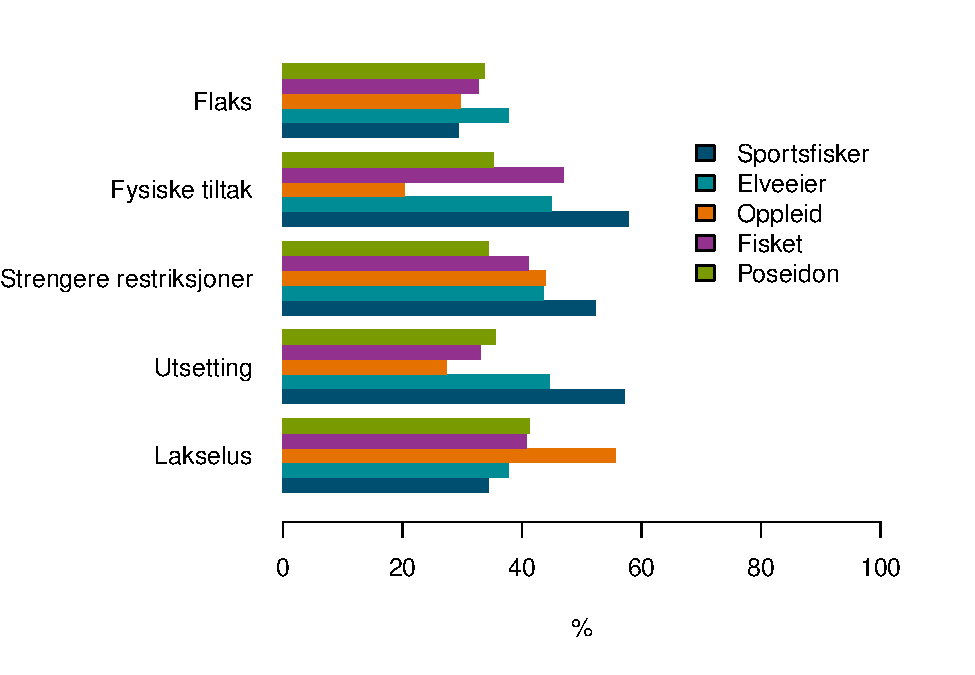
\includegraphics{kortrapport_files/figure-latex/test-chunk2-1.pdf}
\caption{Ett exempel med NINAs grafpalett generert fra R
\label{xy_plot}}
\end{figure}

Bilder kan også legges till slik. Eps-filer angis uten filendelse.

\begin{figure}[htbp]
\centering

\includegraphics{logo}
\caption{Nina-logoen \label{logoen}}
\end{figure}

Her refererer vi til figur \ref{xy_plot}, som er den første figuren vi
lagte. Vi kan også referere til bilder, for eksempel til figur
\ref{logoen}. Notere at man må ha to
\texttt{\textbackslash{}\textbackslash{}} for R-figurer men en
\texttt{\textbackslash{}} for bilder. Dette beteende kan endres i
fremtide versjoner av Pandoc.

\clearpage

\section{Referanser}\label{references}

\setlength{\parindent}{-0.2in} \setlength{\leftskip}{0.2in}
\setlength{\parskip}{8pt} \noindent

\hypertarget{refs}{}
\hypertarget{ref-rmarkdown}{}
Allaire, JJ, Joe Cheng, Yihui Xie, Jonathan McPherson, Winston Chang,
Jeff Allen, Hadley Wickham, Aron Atkins, and Rob Hyndman. 2016.
\emph{Rmarkdown: Dynamic Documents for R}.
\url{http://CRAN.R-project.org/package=rmarkdown}.

\hypertarget{ref-rticles}{}
Allaire, JJ, R Foundation, Hadley Wickham, Journal of Statistical
Software, Yihui Xie, Ramnath Vaidyanathan, Assocation for Computing
Machinery, et al. 2016. \emph{Rticles: Article Formats for R Markdown}.

\hypertarget{ref-NinaR}{}
Astrom, Jens. 2016. \emph{NinaR: Document Templates and Functions for
NINA}.

\hypertarget{ref-Pedersen2016}{}
Pedersen, Follestad, C. H. 2016. ``Statusoversikt for Jaktbart
Småvilt.'' \emph{NINA Rapport} 1178: 258s.


%\clearpage
%\fancyhf{}
%\newgeometry{a4paper, bottom=8cm, top=2cm, left=1.5cm, right=1.5cm}
%\pagestyle{endfooter}

\end{document}
